% ================================================================
% PRESENTATION BEAMER — Battle Météorage 2026
% GBS Survival Analysis — Version lisible, rien ne déborde
% ================================================================
\documentclass[aspectratio=169,t,11pt]{beamer}

\usepackage[T1]{fontenc}
\usepackage[utf8]{inputenc}
\usepackage[french]{babel}
\usepackage{lmodern}
\usepackage{amsmath,amssymb}
\usepackage{booktabs}
\usepackage{array}
\usepackage{tikz}
\usetikzlibrary{arrows.meta,decorations.pathreplacing,calc}
\usepackage[most]{tcolorbox}
\usepackage{xcolor}
\usepackage{graphicx}
\graphicspath{{notebooks/}{results/}{_archive/}}

% ── Couleurs ────────────────────────────────────────────────────
\definecolor{metBlue}{RGB}{14,52,100}
\definecolor{metMid}{RGB}{46,117,182}
\definecolor{metLight}{RGB}{191,215,237}
\definecolor{metGreen}{RGB}{10,150,100}
\definecolor{metOrange}{RGB}{210,110,0}
\definecolor{metRed}{RGB}{190,45,45}

% ── Thème ───────────────────────────────────────────────────────
\usetheme{Boadilla}
\setbeamertemplate{navigation symbols}{}
\setbeamercolor{structure}{fg=metBlue}
\setbeamercolor{frametitle}{bg=metBlue,fg=white}
\setbeamercolor{block title}{bg=metMid,fg=white}
\setbeamercolor{block body}{bg=metLight!25}
\setbeamercolor{block title alerted}{bg=metRed,fg=white}
\setbeamercolor{block body alerted}{bg=metRed!8}
\setbeamercolor{block title example}{bg=metGreen,fg=white}
\setbeamercolor{block body example}{bg=metGreen!10}
\setbeamerfont{frametitle}{size=\large,series=\bfseries}

\setbeamertemplate{headline}{%
  \begin{beamercolorbox}[wd=\paperwidth,ht=2pt]{palette primary}\end{beamercolorbox}}
\setbeamertemplate{footline}{%
  \begin{beamercolorbox}[wd=\paperwidth,ht=15pt,dp=4pt,
    leftskip=8pt,rightskip=8pt]{palette secondary}%
    \small\color{white}Battle Météorage 2026 · GBS Survival Analysis%
    \hfill\insertframenumber/\inserttotalframenumber\hspace{4pt}%
  \end{beamercolorbox}}

% ── Réduction marges des blocs ──────────────────────────────────
\setbeamersize{text margin left=7pt,text margin right=7pt}
\addtobeamertemplate{block begin}{}{\vspace{-2pt}}
\addtobeamertemplate{block end}{\vspace{-2pt}}{}

% ── tcolorbox compact ───────────────────────────────────────────
\tcbset{mybox/.style={
  arc=3pt,boxrule=1pt,
  top=3pt,bottom=3pt,left=5pt,right=5pt,
  fonttitle=\small\bfseries}}

% ================================================================
\title[GBS Battle Météorage]{\textbf{Battle Météorage 2026}\\[0.3em]
  \large Gradient Boosting Survival Analysis}
\subtitle{Prédiction de fin d'alertes foudre aéroportuaires}
\author{Data Battle 2026}
\date{}

\begin{document}

% ── TITRE ───────────────────────────────────────────────────────
{
\setbeamertemplate{footline}{}
\setbeamertemplate{headline}{}
\begin{frame}[plain]
\begin{tikzpicture}[remember picture,overlay]
  \fill[metBlue] (current page.south west) rectangle (current page.north east);
  \fill[metGreen] ([yshift=-1pt]current page.north west)
    rectangle ([yshift=5pt]current page.north east);
  \fill[metMid!50] (current page.south west)
    rectangle ([yshift=2.4cm]current page.south east);
  \node[font=\LARGE\bfseries,text=white,anchor=center]
    at ([yshift=1.8cm]current page.center) {Battle Météorage 2026};
  \node[font=\large,text=white,anchor=center]
    at ([yshift=0.9cm]current page.center) {Gradient Boosting Survival Analysis};
  \node[font=\normalsize,text=metLight,anchor=center]
    at ([yshift=0.1cm]current page.center)
    {Prédiction de fin d'alertes foudre aéroportuaires};
  \draw[metGreen,line width=2pt]
    ([xshift=2.5cm]current page.west|-current page.center)
    -- ([xshift=-2.5cm]current page.east|-current page.center);
  \node[font=\small,text=metLight!70!white,anchor=center]
    at ([yshift=-1.4cm]current page.center)
    {Approche complémentaire, suite du rapport Weibull AFT};
\end{tikzpicture}
\end{frame}
}

% ── PLAN ────────────────────────────────────────────────────────
\begin{frame}{Plan de la présentation}
  \footnotesize
  \tableofcontents
\end{frame}

% ================================================================
\section{Contexte opérationnel}
% ================================================================

\begin{frame}{Le problème : règle Météorage actuelle}
\vspace{-2pt}
\begin{columns}[T]

\column{0.45\textwidth}
\begin{block}{Règle en production}
\small
Une alerte foudre est levée \textbf{30 min après le dernier éclair
nuage-sol} dans un rayon de 20 km autour de l'aéroport.\\[3pt]
Chaque nouvel éclair \textbf{remet le compteur à zéro}.
\end{block}
\vspace{4pt}
\begin{alertblock}{Conséquence opérationnelle}
\small
Aéroport fermé tant que des éclairs surviennent, et 30 min de plus
après le dernier, \textbf{même si l'orage est déjà terminé}.\\[3pt]
Coût : immobilisation des opérations sol, retards passagers.
\end{alertblock}

\column{0.52\textwidth}
\vspace{4pt}
\begin{tikzpicture}[xscale=0.7,yscale=0.9]
  \draw[-{Stealth},thick,metBlue] (-0.1,0) -- (7.6,0)
    node[right,font=\footnotesize]{temps};
  \foreach \x in {0.5,1.2,2.0,2.9,3.8,4.7,5.5} {
    \draw[metOrange,line width=1.2pt] (\x,0.05) -- (\x,0.55);
    \node[metOrange,font=\footnotesize] at (\x,0.75) {$\star$};
  }
  \draw[metRed,line width=2pt] (5.5,0.05) -- (5.5,0.55);
  \node[metRed,font=\scriptsize\bfseries,above] at (5.5,0.78) {dernier CG};
  \draw[decorate,decoration={brace,amplitude=3pt},metBlue,thick]
    (0.5,1.0) -- (5.5,1.0)
    node[midway,above=3pt,font=\footnotesize,metBlue]{\textbf{durée de l'orage}};
  \draw[metGreen,line width=2pt] (6.3,0.05) -- (6.3,-0.4);
  \node[metGreen,font=\scriptsize\bfseries,below]
    at (6.3,-0.4) {$t_{\mathrm{pred}}$};
  \draw[metOrange,line width=2pt] (7.3,0.05) -- (7.3,-0.4);
  \node[metOrange,font=\scriptsize\bfseries,below]
    at (7.3,-0.4) {$t_{\mathrm{règle}}$};
  \fill[metGreen!30] (6.3,-0.25) rectangle (7.3,0.05);
  \node[metGreen!70!black,font=\scriptsize\bfseries] at (6.8,-0.1) {gain};
\end{tikzpicture}
\vspace{4pt}
\begin{exampleblock}{Objectif du projet}
\footnotesize
\textbf{Réduire la durée d'attente} sous la contrainte
\textbf{risque $< 2\,\%$} qu'un éclair $<3$ km survienne après la levée.
\end{exampleblock}
\end{columns}
\end{frame}

% ================================================================
\section{Les données}
% ================================================================

\begin{frame}{Les données fournies par Météorage}
\vspace{-2pt}
\begin{columns}[T]

\column{0.42\textwidth}
\begin{block}{Source}
\small
Une ligne $=$ \textbf{un éclair nuage-sol (CG)} détecté dans un rayon de
20 km autour d'un aéroport.\\[3pt]
\textbf{5 aéroports} : Ajaccio, Bastia, Biarritz, Nantes, Pise.
\end{block}
\vspace{4pt}
\begin{block}{Volumes}
\small
\begin{tabular}{lrr}
\toprule
\textbf{Période} & \textbf{Éclairs CG} & \textbf{Alertes} \\
\midrule
Train  2016-2020 & 41\,509  & $\sim$2\,200 \\
Test   2021-2022 & 15\,090  & $\sim$800    \\
Jury   2023-2025 & 80\,186  & 1\,352       \\
\bottomrule
\end{tabular}
\end{block}

\column{0.56\textwidth}
\begin{block}{Colonnes clés}
\footnotesize
\begin{tabular}{ll}
\toprule
\textbf{Colonne} & \textbf{Description} \\
\midrule
\texttt{date}              & Horodatage UTC de l'éclair \\
\texttt{dist}              & Distance à l'aéroport (km) \\
\texttt{amplitude}         & Courant de décharge (kA, signé) \\
\texttt{icloud}            & Booléen : éclair intra-nuage (écarté) \\
\texttt{airport\_alert\_id} & ID unique de l'alerte en cours \\
\texttt{airport}           & Aéroport concerné \\
\bottomrule
\end{tabular}
\end{block}
\vspace{4pt}
\begin{alertblock}{Choix méthodologique}
\footnotesize
On ne garde \textbf{que les CG} (les intra-nuage \texttt{icloud=True}
ne sont pas considérés dangereux pour les opérations sol).
\end{alertblock}
\end{columns}
\end{frame}

% ================================================================
\section{Exploration des données}
% ================================================================

\begin{frame}{Exploration : où et quand frappent les éclairs ?}
\vspace{-4pt}
\begin{center}
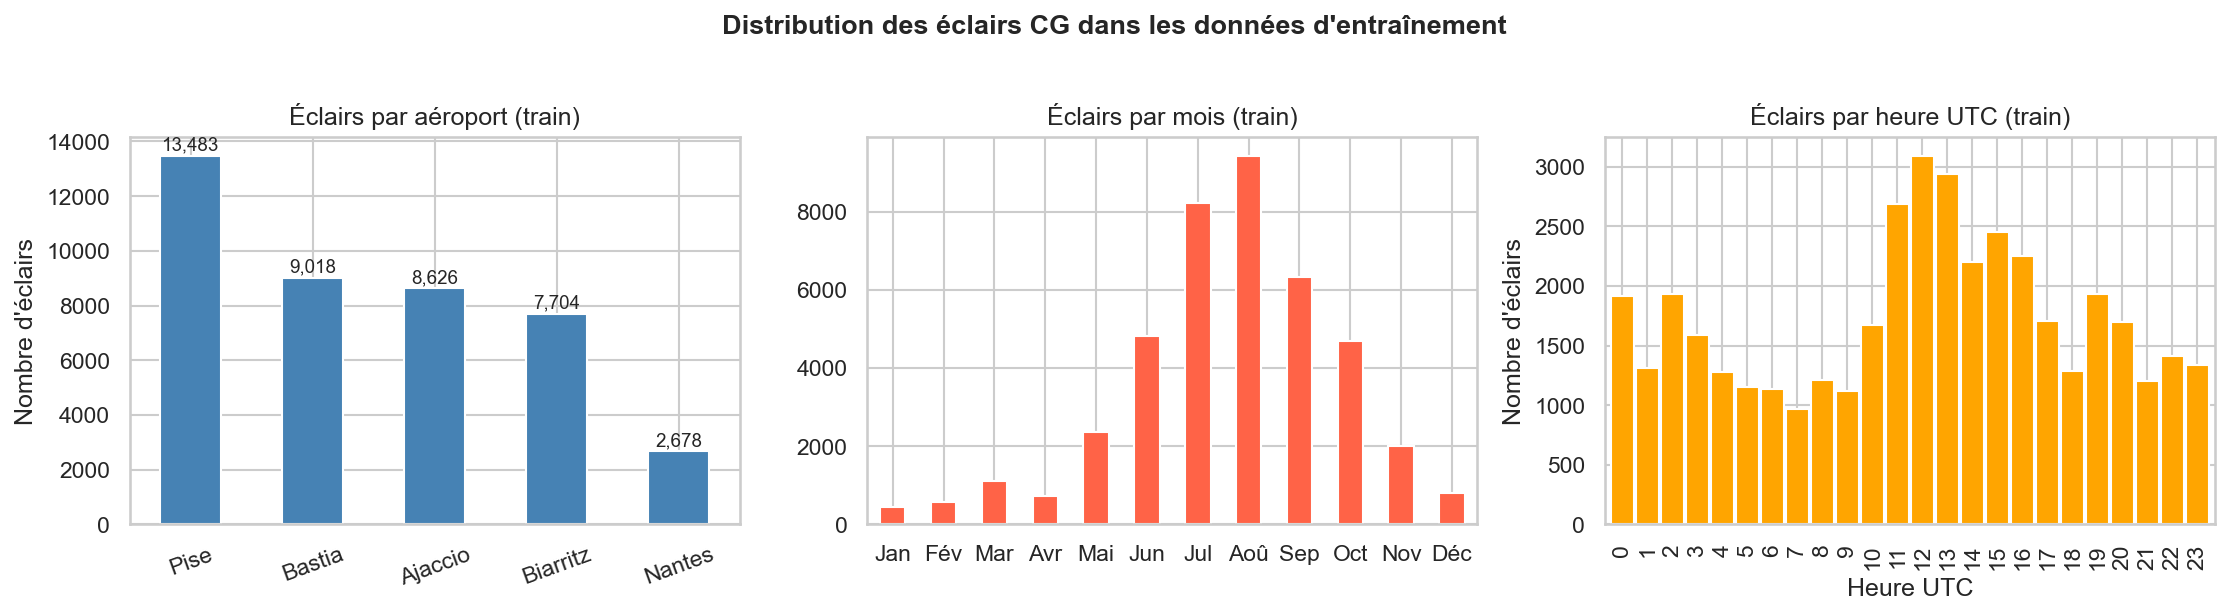
\includegraphics[width=0.97\textwidth]{distrib_eclairs.png}
\end{center}
\vspace{-6pt}
\begin{columns}[T]
\column{0.33\textwidth}
\begin{tcolorbox}[mybox,colback=metMid!10,colframe=metMid,title={Aéroport}]
\footnotesize
Pise (13\,483) $\gg$ Nantes (2\,678).\\
Ratio \textbf{5$\times$}.\\
$\Rightarrow$ feature \texttt{airport\_enc}.
\end{tcolorbox}
\column{0.33\textwidth}
\begin{tcolorbox}[mybox,colback=metOrange!10,colframe=metOrange,title={Saison}]
\footnotesize
Pic juillet-août.\\
$>60$\,\% des éclairs sur 3 mois.\\
$\Rightarrow$ feature \texttt{doy\_sin/cos}.
\end{tcolorbox}
\column{0.33\textwidth}
\begin{tcolorbox}[mybox,colback=metGreen!10,colframe=metGreen,title={Heure}]
\footnotesize
Pic 12-15h UTC.\\
Convection diurne.\\
$\Rightarrow$ feature \texttt{h\_sin/cos}.
\end{tcolorbox}
\end{columns}
\end{frame}

\begin{frame}{Exploration : durée et intensité des orages}
\vspace{-4pt}
\begin{center}
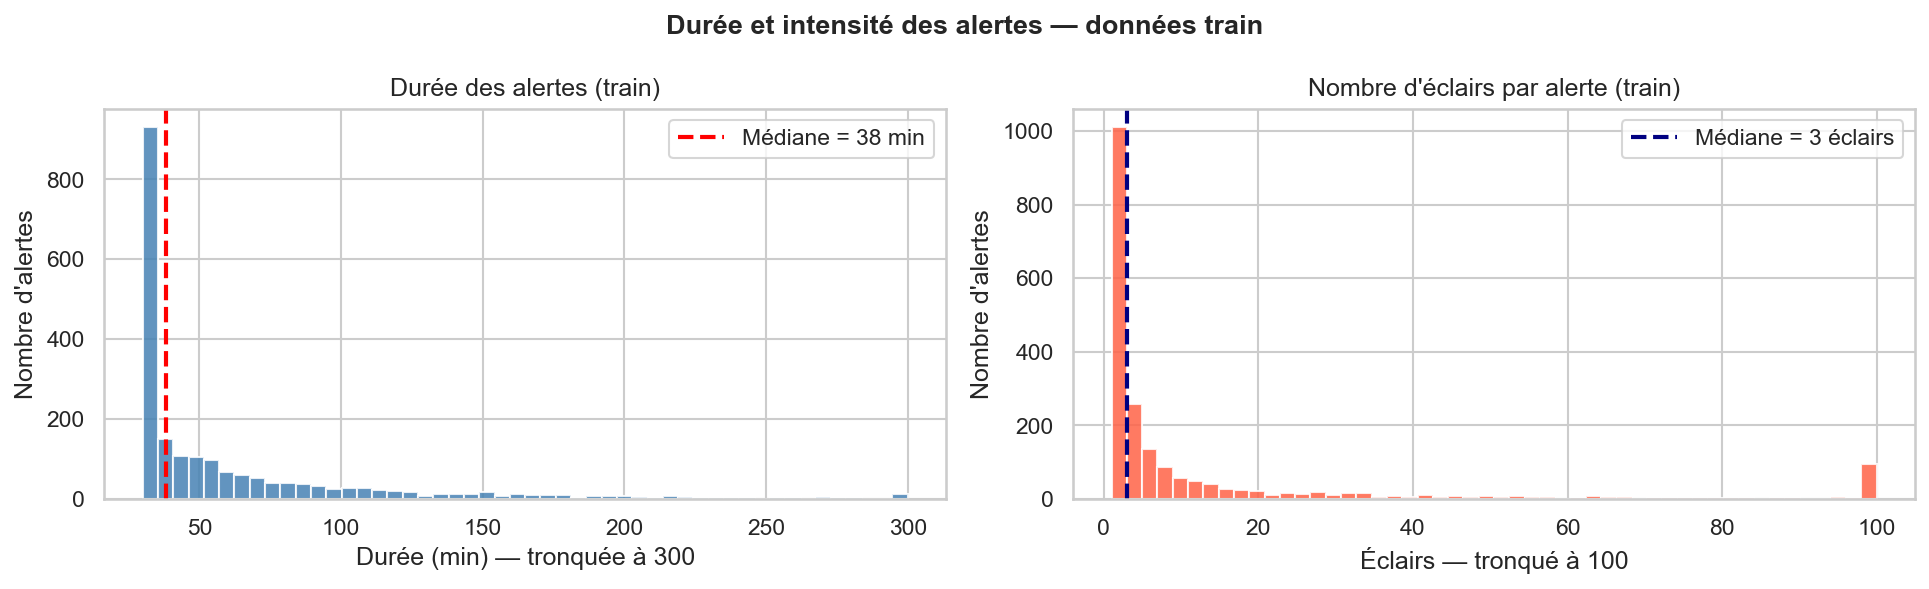
\includegraphics[width=0.95\textwidth]{duree_alertes.png}
\end{center}
\vspace{-4pt}
\begin{columns}[T]
\column{0.50\textwidth}
\begin{block}{Durée d'orage = premier CG $\to$ dernier CG}
\scriptsize
\begin{tabular}{lr}
Médiane durée orage    & \textbf{38 min} \\
Q75 durée              & 60 min \\
Médiane nb éclairs     & \textbf{3} \\
Q75 nb éclairs         & 9 \\
\end{tabular}\\[3pt]
\textit{Attention} : durée d'alerte officielle $=$ durée d'orage $+$ 30 min de fermeture.
\end{block}
\column{0.46\textwidth}
\begin{exampleblock}{Constat}
\scriptsize
Distribution \textbf{très asymétrique} : moitié des orages $<40$ min, 3 éclairs.
La règle des 30 min ajoute donc une attente quasi égale à la durée moyenne d'un orage.
\end{exampleblock}
\end{columns}
\end{frame}

\begin{frame}{Synthèse de l'exploration : opportunité d'optimisation}
\vspace{-2pt}
\begin{tcolorbox}[mybox,colback=metBlue!5,colframe=metBlue,
  title={Trois constats forts ressortent des données}]
\small
\begin{enumerate}\setlength\itemsep{2pt}
  \item \textbf{Hétérogénéité spatiale} entre aéroports (ratio 5$\times$ entre Pise et Nantes)
        $\Rightarrow$ un modèle doit conditionner sur l'aéroport.
  \item \textbf{Périodicités fortes} (saison, heure du jour) $\Rightarrow$
        encodage cyclique nécessaire pour les arbres de décision.
  \item \textbf{Alertes courtes en majorité} (médiane 38 min, 3 éclairs)
        $\Rightarrow$ la règle 30 min impose souvent une attente injustifiée.
\end{enumerate}
\end{tcolorbox}
\vspace{4pt}
\begin{exampleblock}{Conclusion de l'exploration}
\small
Il existe une \textbf{marge d'optimisation réelle} : un modèle qui exploite
ces régularités peut prédire la fin d'orage plus tôt, sans compromis sur la sécurité,
dès lors qu'on quantifie l'incertitude.\\[4pt]
$\Rightarrow$ Cadre statistique adapté : \textbf{l'analyse de survie}, qui modélise
la durée jusqu'à un événement avec censure.
\end{exampleblock}
\end{frame}

% ================================================================
\section{Formalisation mathématique}
% ================================================================

\begin{frame}{Formalisation : variable cible et censure}
\vspace{-2pt}
\begin{columns}[T]

\column{0.50\textwidth}
\begin{block}{Variable cible $T_i$}
\footnotesize
Pour chaque éclair $i$ : $T_i$ = délai (min) jusqu'au prochain CG de la même alerte.\\[3pt]
\textbf{Censure à droite} : si l'alerte se ferme avant un nouvel
éclair, on sait seulement que $T_i \ge 30$ min.
$\delta_i \in \{0,1\}$ : indicateur d'événement ($1$ = observé, $0$ = censuré).
\end{block}
\vspace{2pt}
\begin{alertblock}{Vérification empirique (train)}
\footnotesize
\textbf{95,4\,\%} événements observés, \textbf{4,6\,\%} censurés.
La censure existe et doit être traitée correctement.
\end{alertblock}

\column{0.46\textwidth}
\begin{tcolorbox}[mybox,colback=metMid!10,colframe=metMid,
  title={Hypothèses du modèle}]
\footnotesize
\textbf{H1.} La censure est \textbf{non-informative} : la fermeture
de l'alerte est indépendante du temps de survie résiduel.\\[3pt]
\textbf{H2.} Les éclairs d'une même alerte sont traités comme des
observations conditionnellement indépendantes, étant donné le
contexte $x_i$ (features).\\[3pt]
\textbf{H3.} Le processus est \textbf{stationnaire conditionnellement} :
le risque à un instant donné ne dépend que de $x_i$, pas du temps absolu.\\[3pt]
\textbf{H4.} (Cox PH) Les covariables ont un effet
\textbf{multiplicatif} sur le risque instantané.
\end{tcolorbox}
\end{columns}
\end{frame}

\begin{frame}{Fonctions clés en analyse de survie}
\vspace{-2pt}
\begin{columns}[T]

\column{0.55\textwidth}
\begin{block}{Trois quantités équivalentes}
\footnotesize
\textbf{Fonction de survie} : $\;S(t) = \mathbb{P}(T > t)$, $S(0)=1$, $S(\infty)=0$.\\[3pt]
\textbf{Fonction de hasard} (risque instantané) :
\[ \lambda(t) = \lim_{dt \to 0} \frac{\mathbb{P}(t \le T < t+dt \mid T \ge t)}{dt}. \]
\textbf{Hasard cumulé} :
$\;\Lambda(t) = \int_0^t \lambda(u)\,du$, et $S(t) = e^{-\Lambda(t)}$.
\end{block}
\vspace{2pt}
\begin{exampleblock}{Quantité d'intérêt}
\footnotesize
Conditionné aux features $x_i$ : $\;S(30 \mid x_i) = \mathbb{P}(T_i > 30 \mid x_i)$.\\
Probabilité qu'aucun nouvel éclair ne survienne dans les 30 min suivantes.
\end{exampleblock}

\column{0.42\textwidth}
\vspace{4pt}
\begin{tikzpicture}[xscale=1.1,yscale=1.3]
  \foreach \x in {1,2,3} \draw[gray!25,thin] (\x,0) -- (\x,1.1);
  \foreach \y in {0.3,0.5,1.0} \draw[gray!25,thin] (0,\y) -- (3.3,\y);
  \draw[-{Stealth},thick] (0,0) -- (3.45,0)
    node[right,font=\small]{$t$ (min)};
  \draw[-{Stealth},thick] (0,0) -- (0,1.18)
    node[above,font=\small]{$S(t)$};
  \foreach \x/\l in {1/10,2/20,3/30}
    \node[font=\small,below] at (\x,0) {\l};
  \node[font=\small,left] at (0,1.0) {1};
  \node[font=\small,left] at (0,0.5) {0.5};
  \draw[metGreen,very thick,domain=0:3.0,samples=60]
    plot (\x,{exp(-0.06*\x)});
  \node[metGreen,font=\small\bfseries,right] at (2.5,0.85) {orage calme};
  \draw[metRed,very thick,domain=0:3.0,samples=60]
    plot (\x,{exp(-0.5*\x)});
  \node[metRed,font=\small\bfseries] at (1.4,0.15) {orage actif};
  \draw[metOrange,thick,dashed] (0,0.30) -- (3.3,0.30);
  \node[metOrange,font=\small\bfseries,left] at (0,0.30) {$\theta$};
  \draw[metGreen!70!black,dashed,thick] (2.01,0) -- (2.01,0.30);
  \fill[metGreen!70!black] (2.01,0.30) circle (2.2pt);
  \node[metGreen!70!black,font=\small\bfseries,below] at (2.01,-0.05) {$T^*$};
\end{tikzpicture}
\vspace{2pt}
\begin{center}\footnotesize
Deux $S(t\mid x_i)$ pour des contextes différents.
\end{center}
\end{columns}
\end{frame}

% ================================================================
\section{Modèle non-paramétrique de référence (KM)}
% ================================================================

\begin{frame}{Premier modèle : Kaplan-Meier global}
\vspace{-2pt}
\begin{columns}[T]

\column{0.50\textwidth}
\begin{block}{Estimateur de Kaplan-Meier}
\scriptsize
$\hat{S}_{KM}(t) = \prod_{T_{(k)} \le t} (1 - d_k/n_k)$.
\textbf{Non-paramétrique}, prend en compte la censure.
\end{block}
\vspace{2pt}
\begin{alertblock}{Résultat sur train}
\scriptsize
KM produit une \textbf{courbe globale unique}. À 2\,\% de risque :
$T^\star_{KM} = 28{,}3$ min, gain $= \mathbf{1{,}7}$ min.
\end{alertblock}
\vspace{2pt}
\begin{exampleblock}{Limite $\Rightarrow$ modèle conditionnel}
\scriptsize
Orage calme et actif reçoivent la \textbf{même prédiction}. Il faut $\hat{S}(t \mid x_i)$.
\end{exampleblock}

\column{0.48\textwidth}
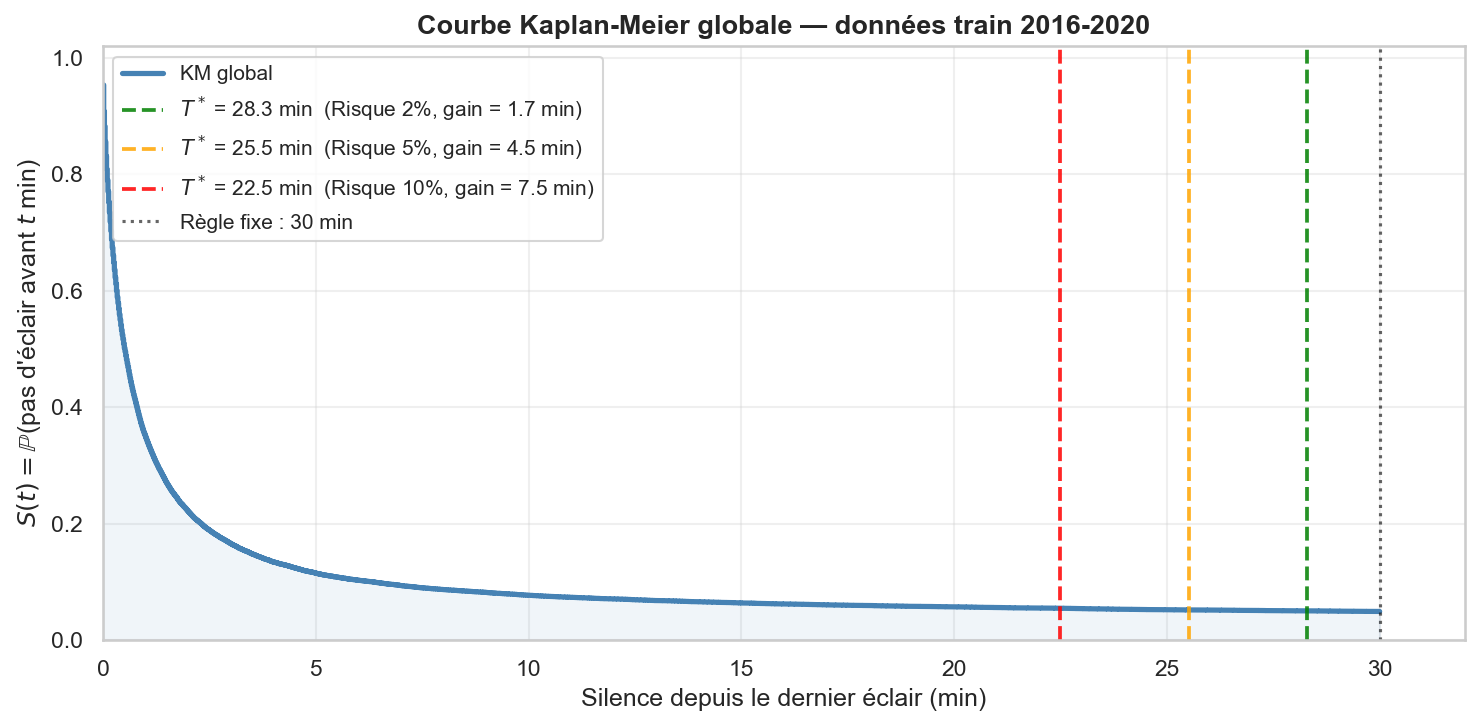
\includegraphics[width=\textwidth]{km_global.png}
\end{columns}
\end{frame}

% ================================================================
\section{Modèle de Cox et Gradient Boosting Survival}
% ================================================================

\begin{frame}{Modèle de Cox à risques proportionnels}
\vspace{-2pt}
\begin{columns}[T]

\column{0.52\textwidth}
\begin{block}{Hypothèse fondamentale (PH)}
\footnotesize
Le risque instantané se factorise :
\[ \lambda(t \mid x_i) = \lambda_0(t) \cdot \exp\!\bigl(f(x_i)\bigr) \]
$\lambda_0(t)$ : risque de base (non spécifié), $f(x_i)$ : score appris.
Conséquence : ratio des hasards indépendant de $t$.
\end{block}
\vspace{2pt}
\begin{block}{Apprentissage de $f$ (vraisemblance partielle)}
\footnotesize
\[
\mathcal{L}(f) = \!\!\sum_{i\,:\,\delta_i = 1}\!\!
\Bigl[ f(x_i) - \log\!\!\sum_{j \in R(T_i)}\!\! e^{f(x_j)} \Bigr]
\]
$R(T_i) = \{j : T_j \ge T_i\}$ : ensemble à risque.
\end{block}

\column{0.46\textwidth}
\begin{exampleblock}{Cox linéaire vs Cox non-linéaire}
\footnotesize
\textbf{Cox linéaire classique} : $f(x_i) = \beta^\top x_i$.
Interprétable, mais incapable de capturer interactions non-linéaires
(saison $\times$ aéroport, etc.).\\[3pt]
\textbf{Notre choix} : $f(x_i)$ appris par un \textbf{ensemble d'arbres boostés} (GBS).
\end{exampleblock}
\vspace{3pt}
\begin{tcolorbox}[mybox,colback=metMid!10,colframe=metMid,
  title={Pourquoi le boosting ?}]
\scriptsize
$\bullet$ Capture interactions et non-linéarités.\\
$\bullet$ Pas d'hypothèse paramétrique sur $\lambda_0(t)$.\\
$\bullet$ Robuste aux features hétérogènes.\\
$\bullet$ Régularisation via profondeur et learning rate.
\end{tcolorbox}
\end{columns}
\end{frame}

\begin{frame}{Algorithme : Gradient Boosting Survival}
\vspace{-2pt}
\begin{columns}[T]

\column{0.55\textwidth}
\begin{tcolorbox}[mybox,colback=metBlue!5,colframe=metBlue,
  title={Boucle d'apprentissage (étape $m = 1, \dots, M$)}]
\footnotesize
\textbf{Initialisation} : $f_0(x) = 0$.\\[3pt]
\textbf{Étape 1.} Calculer le pseudo-résidu (gradient négatif de la
log-vraisemblance partielle évaluée en $f_{m-1}$) :
\[ r_i^{(m)} = -\,\frac{\partial \mathcal{L}}{\partial f(x_i)}\Bigl|_{f = f_{m-1}}. \]
\textbf{Étape 2.} Ajuster un \textbf{arbre de régression} $h_m$
sur les couples $(x_i,\, r_i^{(m)})$.\\[3pt]
\textbf{Étape 3.} Mise à jour avec un pas (learning rate $\nu$) :
\[ f_m(x) = f_{m-1}(x) + \nu \cdot h_m(x). \]
\textbf{Sortie} : $\hat{f}(x) = f_M(x)$.
\end{tcolorbox}

\column{0.43\textwidth}
\begin{block}{Estimateur de Breslow pour $\hat{\Lambda}_0(t)$}
\footnotesize
\[
\hat{\Lambda}_0(t) = \sum_{T_{(k)} \le t}
\frac{\delta_{(k)}}{\sum_{j \in R(T_{(k)})} e^{\hat{f}(x_j)}}
\]
\end{block}
\vspace{3pt}
\begin{exampleblock}{Survie individuelle prédite}
\footnotesize
Pour un nouvel éclair $x_i$ :
\[
\hat{S}(t \mid x_i) = \exp\!\Bigl(-\hat{\Lambda}_0(t)\,e^{\hat{f}(x_i)}\Bigr).
\]
\end{exampleblock}
\vspace{3pt}
\begin{tcolorbox}[mybox,colback=metOrange!10,colframe=metOrange,
  title={Implémentation}]
\scriptsize
\texttt{sksurv.ensemble.}\\\texttt{GradientBoostingSurvivalAnalysis}\\
(\texttt{loss="coxph"}).
\end{tcolorbox}
\end{columns}
\end{frame}

% ================================================================
\section{Construction des features}
% ================================================================

\begin{frame}{Les 13 features construites — un choix justifié}
\vspace{-2pt}
\begin{columns}[T]

\column{0.49\textwidth}
\begin{tcolorbox}[mybox,colback=metMid!10,colframe=metMid,
  title={Temporelles cycliques (5)}]
\scriptsize
$h = $ heure $+$ min$/60$, $d = $ jour de l'année :
$\texttt{h\_cos}=\cos\tfrac{2\pi h}{24}$, $\texttt{h\_sin}=\sin\tfrac{2\pi h}{24}$,
idem \texttt{doy\_cos}, \texttt{doy\_sin}, et \texttt{saison} (1-4).\\[2pt]
\textbf{Pourquoi cyclique :} arbres ne voient pas que 23h et 1h sont proches.
\end{tcolorbox}
\vspace{3pt}
\begin{tcolorbox}[mybox,colback=metOrange!10,colframe=metOrange,
  title={Cadence / fréquence (2)}]
\scriptsize
$\bullet$ \texttt{silence\_min} : délai depuis l'éclair précédent.\\
$\bullet$ \texttt{freq\_5min} : fréquence glissante sur 5 éclairs.\\
\textbf{Signal} : cadence qui ralentit $\Rightarrow$ fin d'orage.
\end{tcolorbox}

\column{0.49\textwidth}
\begin{tcolorbox}[mybox,colback=metGreen!10,colframe=metGreen,
  title={Distance à l'aéroport (3)}]
\scriptsize
$\bullet$ \texttt{dist\_centre} : distance instantanée (km).\\
$\bullet$ \texttt{dist\_avg\_5} : moyenne sur 5 derniers éclairs.\\
$\bullet$ \texttt{dist\_min\_so\_far} : distance min atteinte.\\
\textbf{Signal} : orage qui s'éloigne $\Rightarrow$ alerte qui se termine.
\end{tcolorbox}
\vspace{3pt}
\begin{tcolorbox}[mybox,colback=metRed!10,colframe=metRed,
  title={Contexte alerte / aéroport (3)}]
\scriptsize
$\bullet$ \texttt{rang} : numéro séquentiel dans l'alerte.\\
$\bullet$ \texttt{rang\_norm} : rang normalisé.\\
$\bullet$ \texttt{airport\_enc} : encodage entier aéroport (v7).\\
\textbf{Signal} : aéroport $+$ position conditionnent la survie.
\end{tcolorbox}
\end{columns}
\end{frame}

% ================================================================
\section{Entraînement et calibration des hyperparamètres}
% ================================================================

\begin{frame}{Entraînement du GBS}
\vspace{-2pt}
\begin{columns}[T]

\column{0.50\textwidth}
\begin{block}{Procédure}
\small
\textbf{1.} Données train 2016-2020 (41\,509 éclairs).\\
\textbf{2.} Standardisation des features (\texttt{StandardScaler}).\\
\textbf{3.} \textbf{GridSearch 3-fold} sur la perte de Cox.\\
\textbf{4.} Métrique d'arrêt : \textbf{C-index} sur validation.
\end{block}
\vspace{4pt}
\begin{block}{Hyperparamètres optimisés}
\footnotesize
\begin{tabular}{lll}
\toprule
\textbf{Paramètre} & \textbf{Valeur} & \textbf{Rôle} \\
\midrule
\texttt{n\_estimators}     & 50   & nb d'arbres $M$ \\
\texttt{learning\_rate}    & 0,15 & pas $\nu$ \\
\texttt{max\_depth}        & 3    & complexité arbre \\
\texttt{subsample}         & 0,9  & stochastique \\
\texttt{min\_samples\_leaf}& 10   & régularisation \\
\bottomrule
\end{tabular}
\end{block}

\column{0.46\textwidth}
\begin{exampleblock}{Justification des choix}
\small
\textbf{Arbres peu profonds (depth 3)} : évite le surapprentissage,
les interactions d'ordre élevé sont rares dans ce dataset.\\[3pt]
\textbf{50 arbres, $\nu = 0{,}15$} : couple appris par GridSearch,
compromis entre vitesse et régularisation.\\[3pt]
\textbf{Subsample 0,9} : injecte de la variance, améliore la
généralisation (cf. Friedman 2002).
\end{exampleblock}
\vspace{4pt}
\begin{alertblock}{Coût de calcul}
\footnotesize
Entraînement complet : $\approx 2$ minutes sur CPU pour les 41\,509 éclairs.
\end{alertblock}
\end{columns}
\end{frame}

% ================================================================
\section{Règle de décision et calibration du seuil}
% ================================================================

\begin{frame}{De $\hat{S}(t \mid x_i)$ à la levée d'alerte}
\vspace{-2pt}
\begin{tcolorbox}[mybox,colback=metBlue!5,colframe=metBlue,
  title={Algorithme de décision (seuil $\theta$, ratio $\rho = 0{,}98$)}]
\footnotesize
\textbf{Pour chaque} éclair $x_i$ de l'alerte en cours :
\begin{enumerate}\setlength\itemsep{0pt}
  \item Prédire $\hat{S}(t \mid x_i)$ par le GBS entraîné.
  \item \textbf{Score de confiance} : $\;\mathrm{conf}(x_i) = \hat{S}(30 \mid x_i)$
        — probabilité estimée qu'aucun nouvel éclair n'arrive avant 30 min.
  \item Si $\mathrm{conf}(x_i) > \theta$ : \emph{éclair confiant} $\Rightarrow$
        on calcule l'horizon individuel
        $\;\hat{t}_i = \min\!\bigl\{ t : \hat{S}(t \mid x_i) \le \hat{S}(30 \mid x_i)/\rho \bigr\}.$
  \item Sinon $\hat{t}_i = +\infty$ (le modèle reste inactif).
\end{enumerate}
\vspace{2pt}
\textbf{Décision globale d'alerte} :
\[
t_{\mathrm{pred}} = \min_i \hat{t}_i, \qquad G = \max\!\bigl(0,\; t_{\mathrm{règle}} - t_{\mathrm{pred}}\bigr).
\]
\end{tcolorbox}
\vspace{4pt}
\begin{exampleblock}{Lecture de la règle}
\scriptsize
\textbf{Au moins un} éclair doit être suffisamment confiant pour lever.
On prend le \textbf{minimum} des horizons des éclairs confiants (conservateur).
\end{exampleblock}
\end{frame}

% ================================================================
\section{Évaluation interne et choix de $\theta$}
% ================================================================

\begin{frame}{Métrique principale : le C-index de Harrell}
\vspace{-2pt}
\begin{columns}[T]

\column{0.55\textwidth}
\begin{block}{Définition formelle}
\small
Le C-index mesure la \textbf{concordance} des temps prédits avec les temps observés.
Sur les paires comparables $(i,j)$ avec $T_i < T_j$ et $\delta_i = 1$ :
\[
\mathrm{C} = \frac{\#\{(i,j) : \hat{f}(x_i) > \hat{f}(x_j),\, T_i < T_j,\, \delta_i = 1\}}
                 {\#\{(i,j) : T_i < T_j,\, \delta_i = 1\}}
\]
$\mathrm{C} = 1$ : ordonnancement parfait \quad $\mathrm{C} = 0{,}5$ : aléatoire.
\end{block}
\vspace{3pt}
\begin{exampleblock}{Pourquoi cette métrique}
\footnotesize
$\bullet$ Robuste à la censure (paires non-comparables exclues).\\
$\bullet$ Évalue la \textbf{capacité à ordonner}, ce qui est exactement
ce dont on a besoin pour appliquer un seuil de décision.\\
$\bullet$ Ne dépend pas de la calibration absolue de $\hat{S}$.
\end{exampleblock}

\column{0.43\textwidth}
\begin{tcolorbox}[mybox,colback=metGreen!10,colframe=metGreen,
  title={Résultats validation 2021-2022}]
\small
\centering
\begin{tabular}{lcc}
\toprule
\textbf{Modèle} & \textbf{Train} & \textbf{Test} \\
\midrule
GBS v6 (12 var.) & 0,776 & 0,741 \\
GBS v7 (13 var.) & 0,777 & \textbf{0,742} \\
\bottomrule
\end{tabular}
\end{tcolorbox}
\vspace{4pt}
\begin{tcolorbox}[mybox,colback=metMid!10,colframe=metMid,
  title={Interprétation}]
\scriptsize
$\bullet$ Écart train/test $\le 0{,}003$ : \textbf{pas de surapprentissage}.\\
$\bullet$ 0,742 $\gg$ 0,5 : signal réel capturé.\\
$\bullet$ v7 $\approx$ v6 : \texttt{airport\_enc} améliore surtout la calibration.
\end{tcolorbox}
\end{columns}
\end{frame}

\begin{frame}{Calibration du seuil $\theta$ sur validation}
\vspace{-2pt}
\begin{columns}[T]

\column{0.50\textwidth}
\begin{block}{Procédure de calibration}
\small
On fait varier $\theta \in [0{,}10\,;\,0{,}50]$ et on mesure sur le test 2021-2022 :
\begin{itemize}\setlength\itemsep{1pt}
  \item le \textbf{gain total} (heures économisées),
  \item le \textbf{risque} (\% d'éclairs $<3$ km manqués).
\end{itemize}
\vspace{3pt}
On choisit le $\theta$ qui \textbf{maximise le gain} sous la contrainte
\textbf{risque $< 2\,\%$}.
\end{block}
\vspace{3pt}
\begin{exampleblock}{Choix retenu : $\theta = 0{,}30$}
\footnotesize
$\bullet$ $\theta$ plus bas : modèle plus agressif, risque dépasse 2\,\%.\\
$\bullet$ $\theta$ plus haut : modèle quasi-inactif, peu de gain.\\
$\bullet$ $\theta = 0{,}30$ : compromis optimal sur validation.
\end{exampleblock}

\column{0.46\textwidth}
\begin{tcolorbox}[mybox,colback=metMid!10,colframe=metMid,
  title={Résultats sur test 2021-2022 à $\theta=0{,}30$}]
\small
\centering
\begin{tabular}{lc}
\toprule
\textbf{Métrique} & \textbf{Valeur} \\
\midrule
Alertes évaluées        & $\sim$800 \\
Gain total              & 32 h \\
Gain moyen / alerte     & 4,5 min \\
Risque $<3$ km          & 0,18\,\% \\
\bottomrule
\end{tabular}
\end{tcolorbox}
\vspace{4pt}
\begin{alertblock}{Validation OK}
\footnotesize
Risque très en dessous de la limite 2\,\%, gain non-trivial.\\
$\Rightarrow$ on \textbf{fige} $\theta = 0{,}30$ et le modèle pour
l'évaluation jury sur données 2023-2025 jamais vues.
\end{alertblock}
\end{columns}
\end{frame}

% ================================================================
\section{Protocole et résultats du jury}
% ================================================================

\begin{frame}{Protocole d'évaluation du jury (rappel)}
\vspace{-2pt}
\begin{tcolorbox}[mybox,colback=metBlue!5,colframe=metBlue,
  title={Critère officiel Data Battle 2026}]
\small
\textbf{Donnée d'évaluation} : 80\,186 éclairs CG sur 2023-2025, regroupés en 1\,352 alertes,
\emph{jamais vus} pendant l'entraînement.\\[4pt]
\textbf{Pour chaque alerte}, le jury compare :
\begin{itemize}\setlength\itemsep{1pt}
  \item $t_{\mathrm{règle}}$ : moment de levée selon la règle Météorage (dernier CG + 30 min)
  \item $t_{\mathrm{pred}}$ : moment de levée selon notre modèle
\end{itemize}
\vspace{2pt}
\textbf{Métriques mesurées} :
\[
\text{Gain} = \!\!\sum_{\text{alertes}}\!\! \max\!\bigl(0,\, t_{\mathrm{règle}} - t_{\mathrm{pred}}\bigr),
\qquad
\text{Risque} = \frac{\#\{\text{CG} < 3\text{ km après } t_{\mathrm{pred}}\}}{\#\{\text{CG} < 3\text{ km au total}\}}.
\]
\textbf{Contrainte stricte} : Risque $< 2\,\%$.
\end{tcolorbox}
\vspace{4pt}
\begin{center}
\small\color{metOrange}\textbf{Objectif : maximiser le gain en respectant la contrainte de sécurité.}
\end{center}
\end{frame}

\begin{frame}{Résultats jury 2023-2025 — performance finale}
\vspace{-2pt}

\begin{columns}[c]
\column{0.25\textwidth}
\begin{tcolorbox}[mybox,colback=metMid!10,colframe=metMid,
  halign=center,top=5pt,bottom=5pt]
{\large\bfseries\color{metMid}1\,352}\\[2pt]
\small alertes évaluées
\end{tcolorbox}
\column{0.25\textwidth}
\begin{tcolorbox}[mybox,colback=metGreen!10,colframe=metGreen,
  halign=center,top=5pt,bottom=5pt]
{\large\bfseries\color{metGreen}103{,}5 h}\\[2pt]
\small économisées
\end{tcolorbox}
\column{0.25\textwidth}
\begin{tcolorbox}[mybox,colback=metGreen!10,colframe=metGreen,
  halign=center,top=5pt,bottom=5pt]
{\large\bfseries\color{metGreen}0{,}10\,\%}\\[2pt]
\small risque $<$3 km
\end{tcolorbox}
\column{0.25\textwidth}
\begin{tcolorbox}[mybox,colback=metGreen!10,colframe=metGreen,
  halign=center,top=5pt,bottom=5pt]
{\large\bfseries\color{metGreen}2\,/\,1\,995}\\[2pt]
\small éclairs manqués
\end{tcolorbox}
\end{columns}

\vspace{6pt}
\begin{columns}[T]
\column{0.50\textwidth}
\begin{block}{Détail par version ($\theta=0{,}30$)}
\small
\begin{tabular}{lcc}
\toprule
\textbf{Métrique} & \textbf{v6} & \textbf{v7} \\
\midrule
Gain total          & 105,1 h    & 103,5 h    \\
Gain moy./alerte    & 4,67 min   & 4,59 min   \\
Risque $<3$ km      & 0,10\,\%   & 0,10\,\%   \\
Alertes actives     & $\sim$72\,\% & $\sim$72\,\% \\
\bottomrule
\end{tabular}
\end{block}

\column{0.46\textwidth}
\begin{exampleblock}{Conformité contrainte sécurité}
\small
Risque mesuré $0{,}10\,\%$ contre limite $2\,\%$ :\\
\textbf{20 fois sous la limite officielle.}\\[3pt]
Seuls \textbf{2 éclairs sur 1\,995} ($<3$ km) sont arrivés après notre levée.
\end{exampleblock}
\vspace{4pt}
\begin{alertblock}{Robustesse}
\footnotesize
Performance comparable à validation (test 2021-2022 : 0,18\,\%).\\
Pas de dégradation sur les données jury 2023-2025.
\end{alertblock}
\end{columns}
\end{frame}

% ================================================================
\section{Mise en perspective}
% ================================================================

\begin{frame}{GBS vs Weibull AFT (approche binôme)}
\vspace{-2pt}
\begin{center}
\small
\begin{tabular}{>{\bfseries}lcc}
\toprule
\textbf{Critère} & \textbf{Weibull AFT} & \textbf{GBS CoxPH} \\
\midrule
Type                       & Paramétrique             & Non-paramétrique \\
Forme imposée sur $S(t)$   & $e^{-(t/\lambda(X))^k}$ & Aucune \\
Apprentissage              & MLE direct               & Boosting gradient \\
Gain jury                  & $\sim$330 h              & 103,5 h \\
Risque $<3$ km             & 0,60\,\%                 & \textbf{0,10\,\%} \\
Interprétabilité           & Haute ($\beta$ explicite)& Modérée (importances) \\
Flexibilité                & Faible                   & Haute \\
\bottomrule
\end{tabular}
\end{center}
\vspace{6pt}
\begin{columns}[T]
\column{0.50\textwidth}
\begin{exampleblock}{Complémentarité}
\footnotesize
Weibull \textbf{maximise le gain brut}, GBS \textbf{minimise le risque}.
Un modèle hybride (score GBS $\times$ quantile Weibull) est une piste naturelle.
\end{exampleblock}
\column{0.46\textwidth}
\begin{alertblock}{Limites communes}
\footnotesize
Aucun des deux modèles ne capture la \textbf{structure spatiale 2D}
de l'orage ni sa direction de déplacement. Un modèle spatio-temporel
serait la prochaine étape.
\end{alertblock}
\end{columns}
\end{frame}

% ================================================================
\section{Conclusion}
% ================================================================

\begin{frame}{Conclusion}
\vspace{-2pt}
\begin{columns}[T]

\column{0.56\textwidth}
\begin{exampleblock}{Ce que le GBS apporte}
\small
\begin{itemize}\setlength\itemsep{2pt}
  \item[\checkmark] Une fonction de survie \textbf{individualisée} $\hat{S}(t \mid x_i)$,
                   sans hypothèse paramétrique.
  \item[\checkmark] \textbf{103,5 h économisées} sur jury 2023-2025.
  \item[\checkmark] \textbf{0,10\,\%} de risque, $20\times$ sous la limite de 2\,\%.
  \item[\checkmark] C-index 0,742, écart train/test négligeable.
  \item[\checkmark] Algorithme transparent et reproductible (scikit-survival).
\end{itemize}
\end{exampleblock}
\vspace{4pt}
\begin{alertblock}{Perspectives}
\scriptsize
$\bullet$ Modèle \textbf{hybride} : score GBS $+$ quantile Weibull.
$\bullet$ \textbf{Direction} de déplacement de l'orage. $\bullet$ Features v8 : amplitude, tendance.
\end{alertblock}

\column{0.40\textwidth}
\begin{tcolorbox}[mybox,colback=metBlue!8,colframe=metBlue,
  title={Message clé}]
\small
Le GBS prédit, pour \textbf{chaque éclair}, la probabilité que
l'orage soit terminé. Il lève l'alerte dès qu'un éclair est
suffisamment confiant, avec un seuil $\theta$ calibré pour rester
sous la barre des 2\,\% de risque.
\end{tcolorbox}
\vspace{6pt}
\begin{tcolorbox}[mybox,colback=metGreen!12,colframe=metGreen,
  halign=center,top=6pt,bottom=6pt]
\normalsize\bfseries\color{metGreen}
103,5 h économisées\\[3pt]
0,10\,\% de risque
\end{tcolorbox}
\end{columns}
\end{frame}

% ================================================================
\section{Références}
% ================================================================

\begin{frame}{Références}
\vspace{-4pt}
\begin{block}{Méthodologie statistique}
\scriptsize
\begin{itemize}\setlength\itemsep{0pt}
  \item Cox, D.R. (1972). \textit{Regression Models and Life-Tables}.
    J. R. Stat. Soc. B, 34(2), 187-220.
  \item Kaplan, E.L. \& Meier, P. (1958). \textit{Nonparametric Estimation from
    Incomplete Observations}. JASA, 53(282), 457-481.
  \item Breslow, N. (1972). \textit{Contribution to the discussion of Cox (1972)}.
  \item Harrell, F.E. et al. (1982). \textit{Evaluating the yield of medical tests}.
    JAMA, 247(18), 2543-2546. \hfill (C-index)
  \item Ridgeway, G. (1999). \textit{The state of boosting}.
    Comp. Sci. Stat., 31, 172-181. \hfill (GBM Cox)
  \item Friedman, J. (2001). \textit{Greedy Function Approximation: A Gradient
    Boosting Machine}. Annals of Statistics, 29(5), 1189-1232.
  \item Pölsterl, S. (2020). \textit{scikit-survival: A Library for Time-to-Event
    Analysis Built on Top of scikit-learn}. JMLR, 21(212), 1-6.
\end{itemize}
\end{block}
\vspace{2pt}
\begin{columns}[T]
\column{0.50\textwidth}
\begin{tcolorbox}[mybox,colback=metMid!10,colframe=metMid,title={Logiciels}]
\scriptsize
\textbf{scikit-survival} 0.22 : \texttt{GradientBoostingSurvivalAnalysis}.\\
Python 3.11, pandas, NumPy, Matplotlib, Streamlit.
\end{tcolorbox}
\column{0.50\textwidth}
\begin{tcolorbox}[mybox,colback=metOrange!10,colframe=metOrange,title={Données}]
\footnotesize
Météorage \textit{Data Battle 2026}.\\
56\,599 éclairs CG, 5 aéroports, 2016-2025.\\
Variable cible $T_i$ construite par nos soins.
\end{tcolorbox}
\end{columns}
\end{frame}

% ── MERCI ───────────────────────────────────────────────────────
{
\setbeamertemplate{footline}{}
\setbeamertemplate{headline}{}
\begin{frame}[plain]
\begin{tikzpicture}[remember picture,overlay]
  \fill[metBlue] (current page.south west) rectangle (current page.north east);
  \fill[metGreen] ([yshift=-1pt]current page.north west)
    rectangle ([yshift=5pt]current page.north east);
  \fill[metMid!50] (current page.south west)
    rectangle ([yshift=2.4cm]current page.south east);
  \node[font=\Huge\bfseries,text=white,anchor=center]
    at ([yshift=0.8cm]current page.center) {Merci};
  \node[font=\large,text=metLight,anchor=center]
    at ([yshift=0.0cm]current page.center) {Questions ?};
  \node[font=\small,text=white!60!metBlue,anchor=center]
    at ([yshift=0.7cm]current page.south)
    {Data Battle Météorage 2026 · GBS Gradient Boosting Survival Analysis};
\end{tikzpicture}
\end{frame}
}

\end{document}
